\documentclass{ctexart}
\usepackage{float}
\usepackage{graphicx}
\usepackage{geometry}
\usepackage[hidelinks]{hyperref}
\usepackage{caption}
\usepackage{subcaption}
\usepackage{amsmath}
\usepackage{fancyhdr}
\usepackage{xcolor}
\usepackage{fontspec}
\usepackage{listings}[language=c,numberstyle=\tiny,basicstyle=\small]
\definecolor{codegreen}{rgb}{0,0.6,0}
\definecolor{codegray}{rgb}{0.5,0.5,0.5}
\definecolor{codepurple}{rgb}{0.58,0,0.82}
\definecolor{backcolour}{rgb}{0.95,0.95,0.92}
% \renewcommand{\figurename}{Figure}
% \renewcommand{\today}{\number\year, \number\month, \number\day}
%页面参数
%页边距
\geometry{top=1in,bottom=1in,left=2cm,right=2cm}
%行距
\linespread{1.5}
%目录深度
\setcounter{secnumdepth}{3}
%
% \renewcommand {\thetable} {\thesection{}.\arabic{table}}
% \renewcommand {\thefigure} {\thesection{}.\arabic{figure}}
\pagestyle{fancy}
\lstset{ %
backgroundcolor=\color{white},   % choose the background color
basicstyle=\footnotesize\ttfamily,        % size of fonts used for the code
columns=fullflexible,
breaklines=true,                 % automatic line breaking only at whitespace
captionpos=b,                    % sets the caption-position to bottom
tabsize=4,   % comment style
escapeinside={\%*}{*)},          % if you want to add LaTeX within your code
keywordstyle=\color{blue},       % keyword style
frame=single,
rulesepcolor=\color{red!20!green!20!blue!20},
% identifierstyle=\color{red},
language=c,
}
\chead{\textcolor{red}{A}dvanced Honor \textcolor{red}{C}lass of \textcolor{red}{E}ngineering \textcolor{red}{E}ducation}
\lhead{}
\rhead{}
\begin{document}
\setcounter{section}{3}
\section*{Part 3}
\begin{figure}[H]
  \centering
  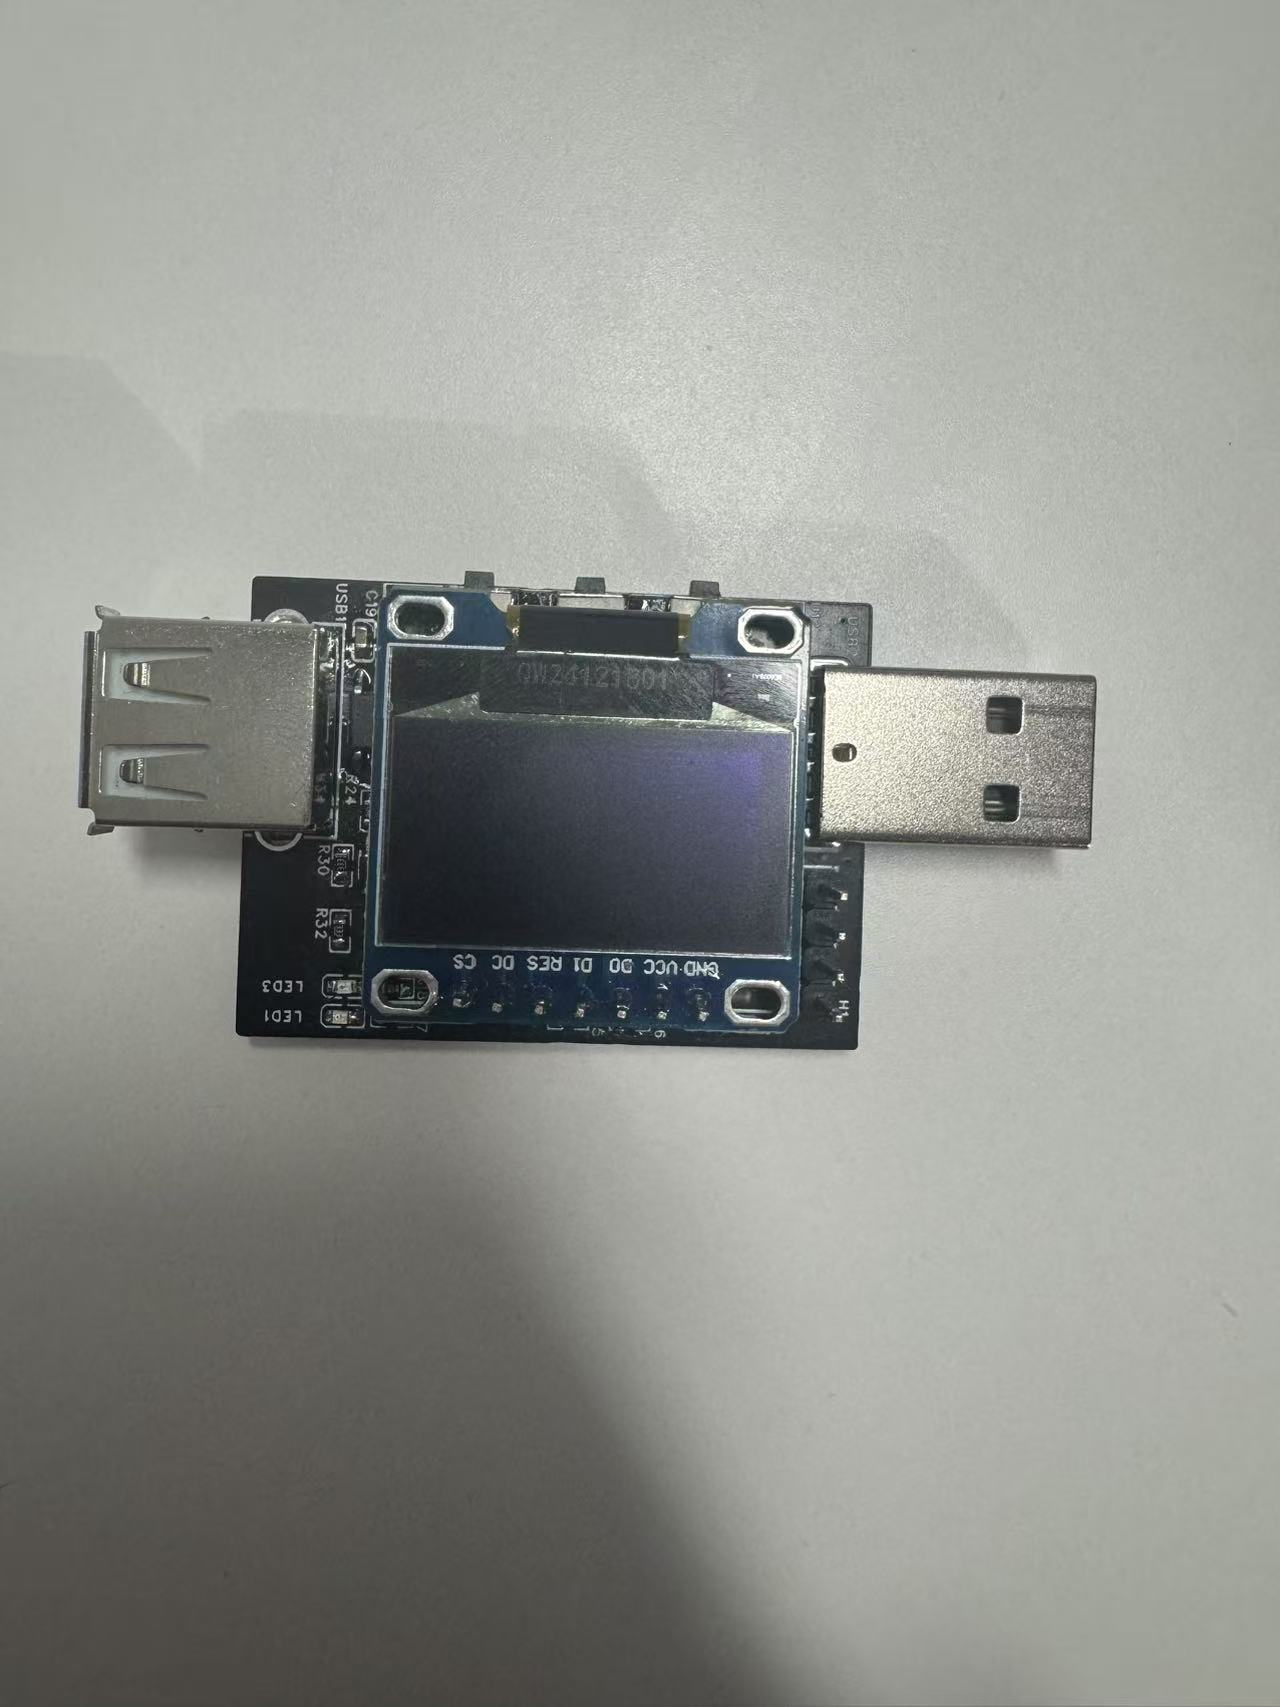
\includegraphics[width = .5\textwidth]{./figures/z.jpg}\\
  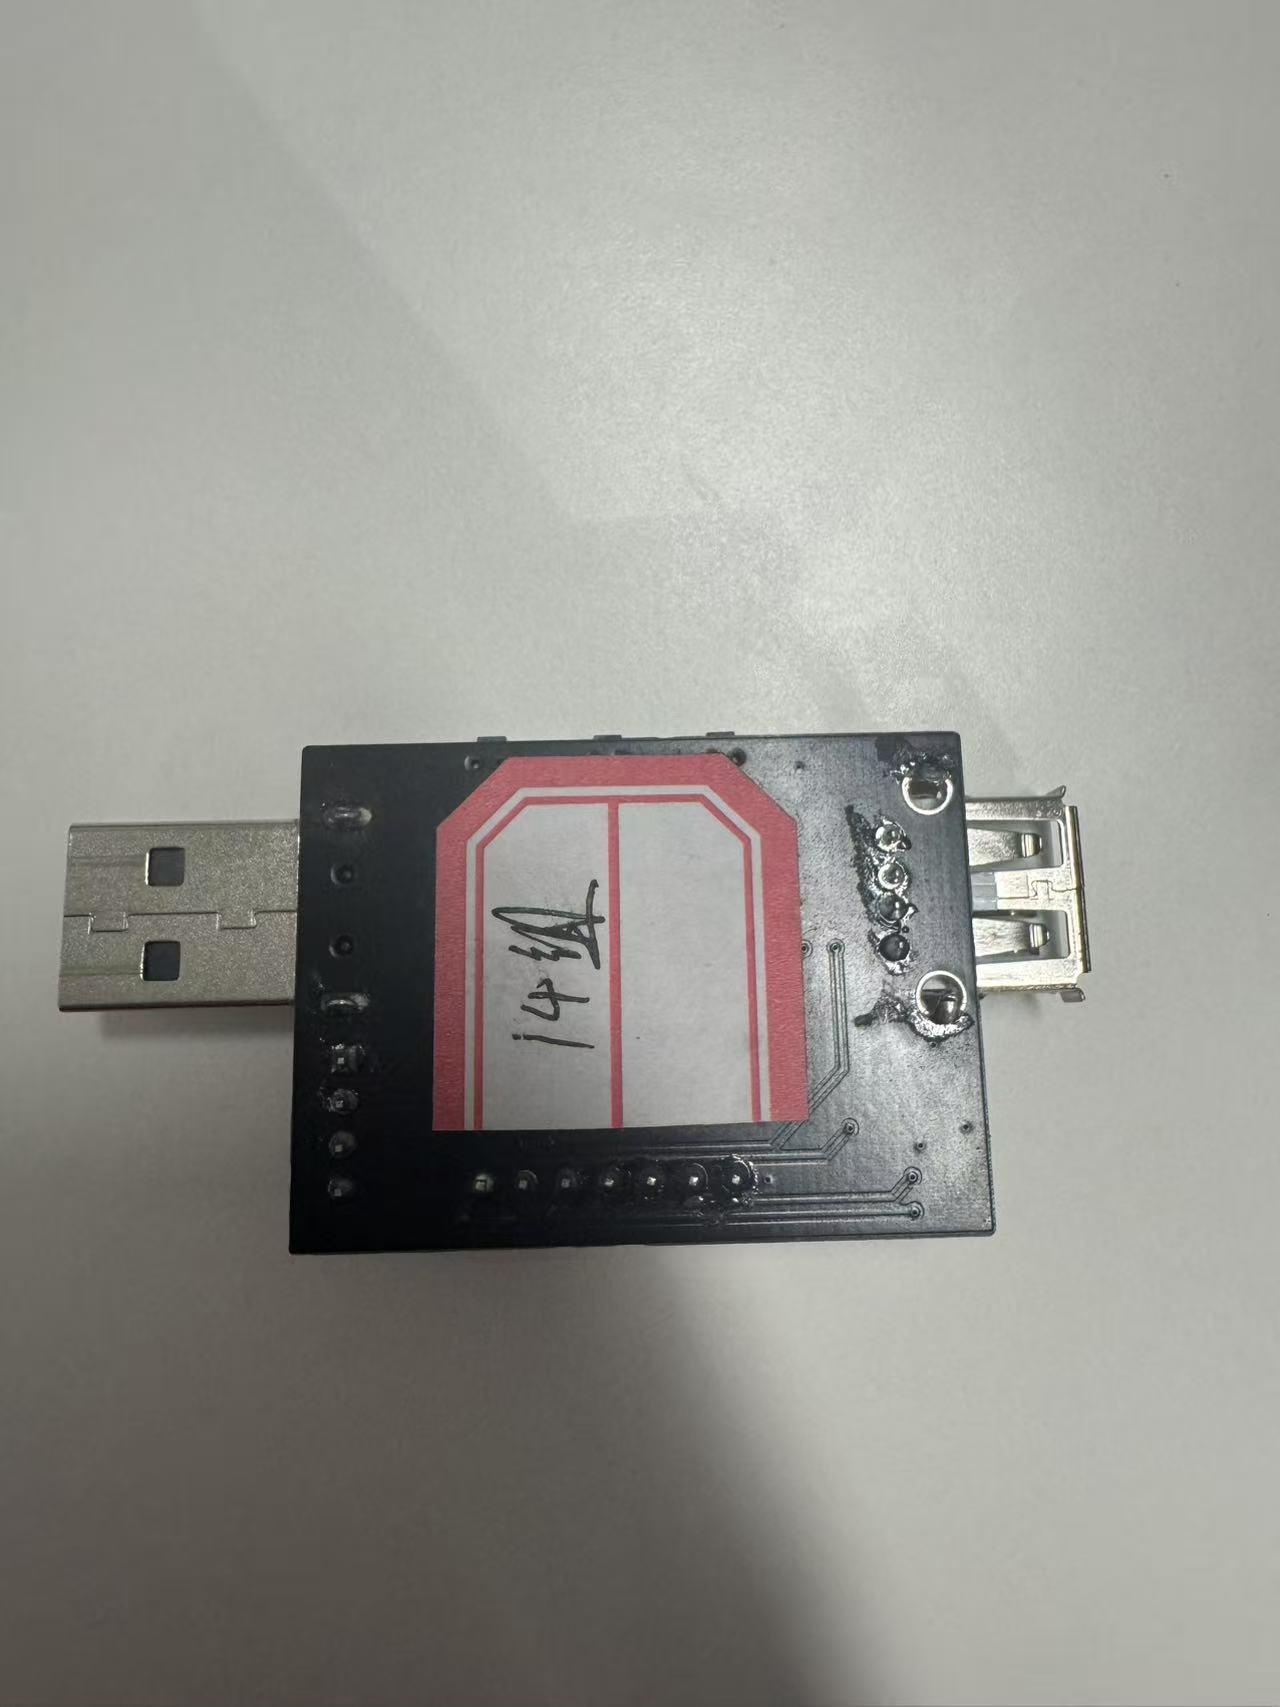
\includegraphics[width = .5\textwidth]{./figures/f.jpg}
  \caption{焊接好的板子正反面}
\end{figure}
由于上过电子工程训练,所以对焊接并不太陌生,但是这次使用的刀型焊枪使用不太习惯。

焊接芯片时使用了拖焊的方式,有时会发生连焊,加上助焊剂会好很多。
\section*{Part 4}
\subsection{Hello,world}
首先我们焊接之后得到单片机,通过ST-Link将Vcc,Swim,GND,Nrst与芯片的对应针脚用杜邦线连接,就可以在iar软件中进行烧录。

但我们在烧录的过程中出现了报错,我们的iar无法检测到swim端口,导致代码无法烧录。后来,通过查阅PCB线路图,发现Vcd为3.3V,而Vcc为5V,故重新将
板子以5V电压供电,并将iar工程中的芯片型号,debug工具设置为stm8s003F3与stlink,并将led管脚设置为pc6,终于将板子点亮。

\begin{figure}[H]
\centering
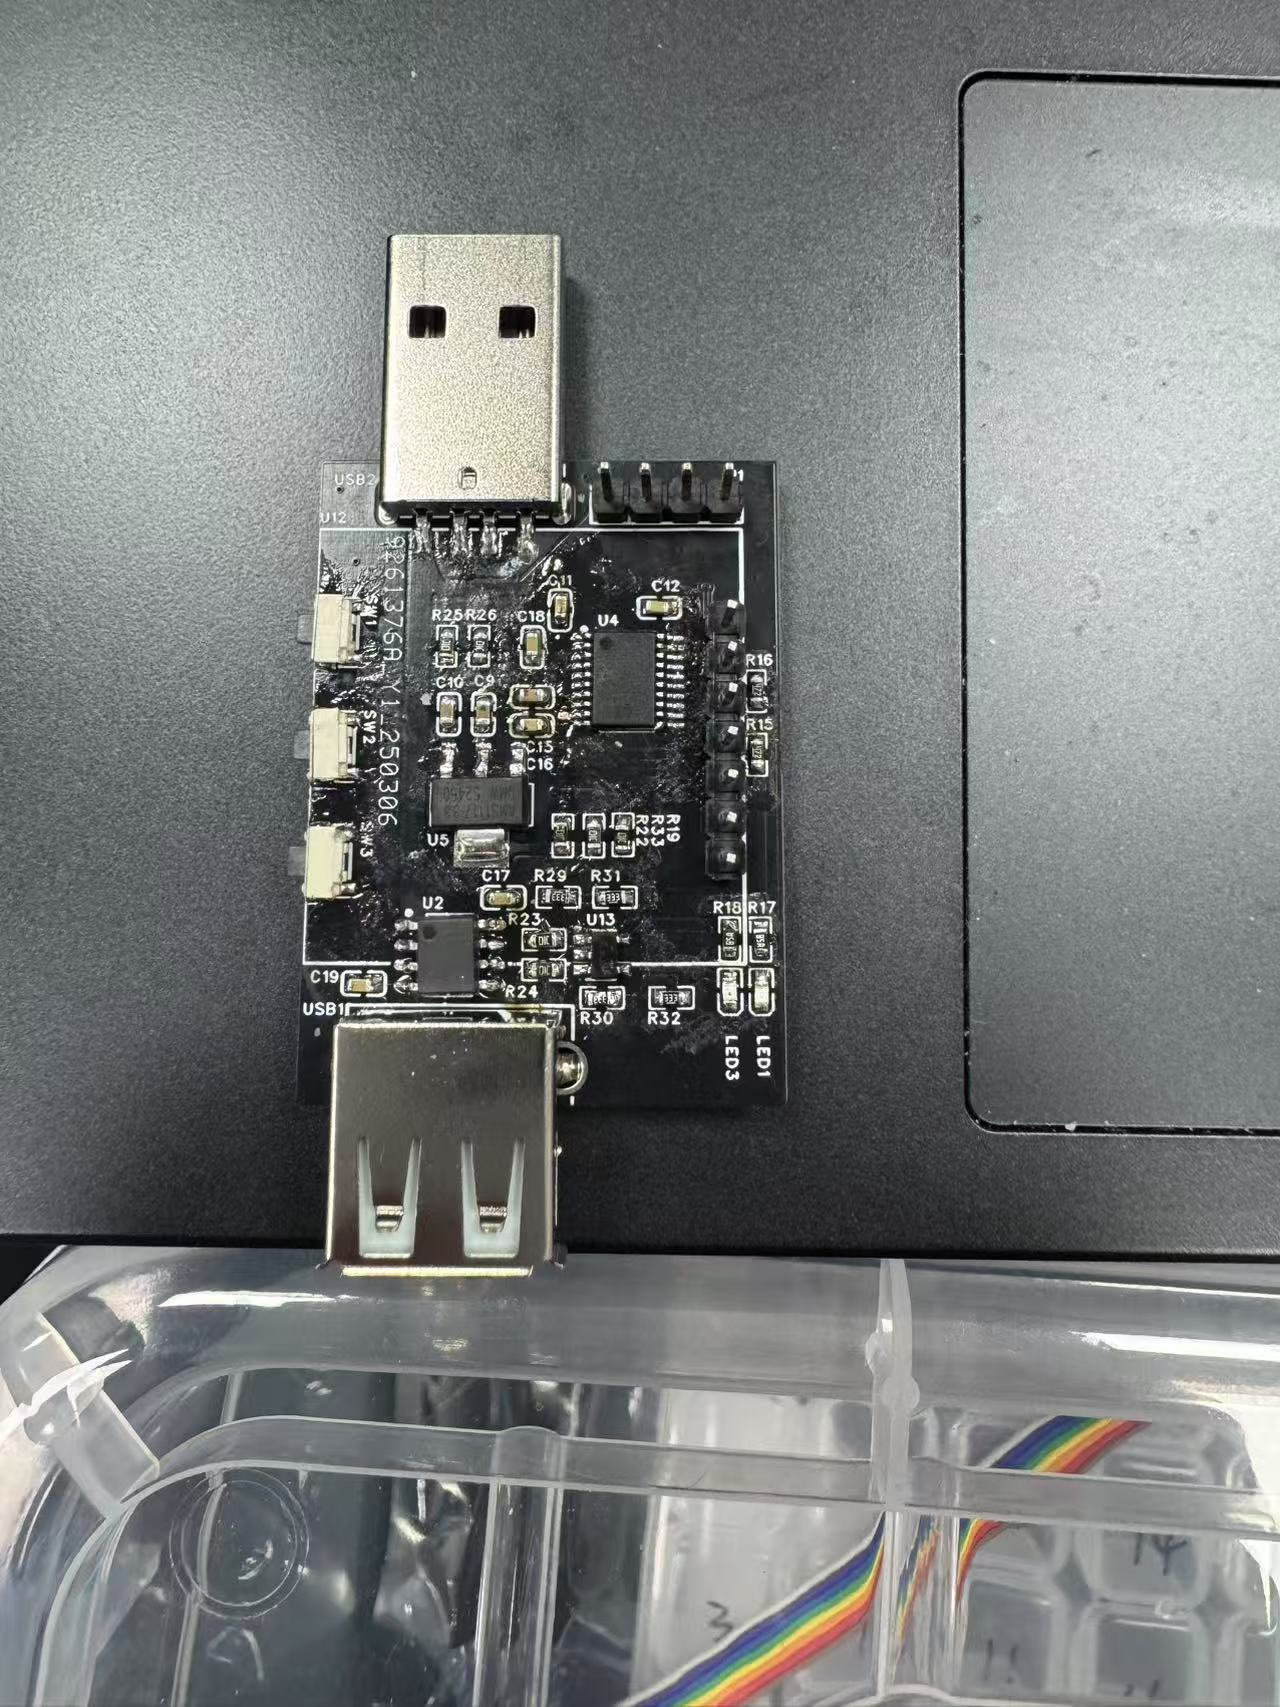
\includegraphics[width = .2\textwidth]{./figures/c9c82cc123bb287693d88c08433309e.jpg}\\
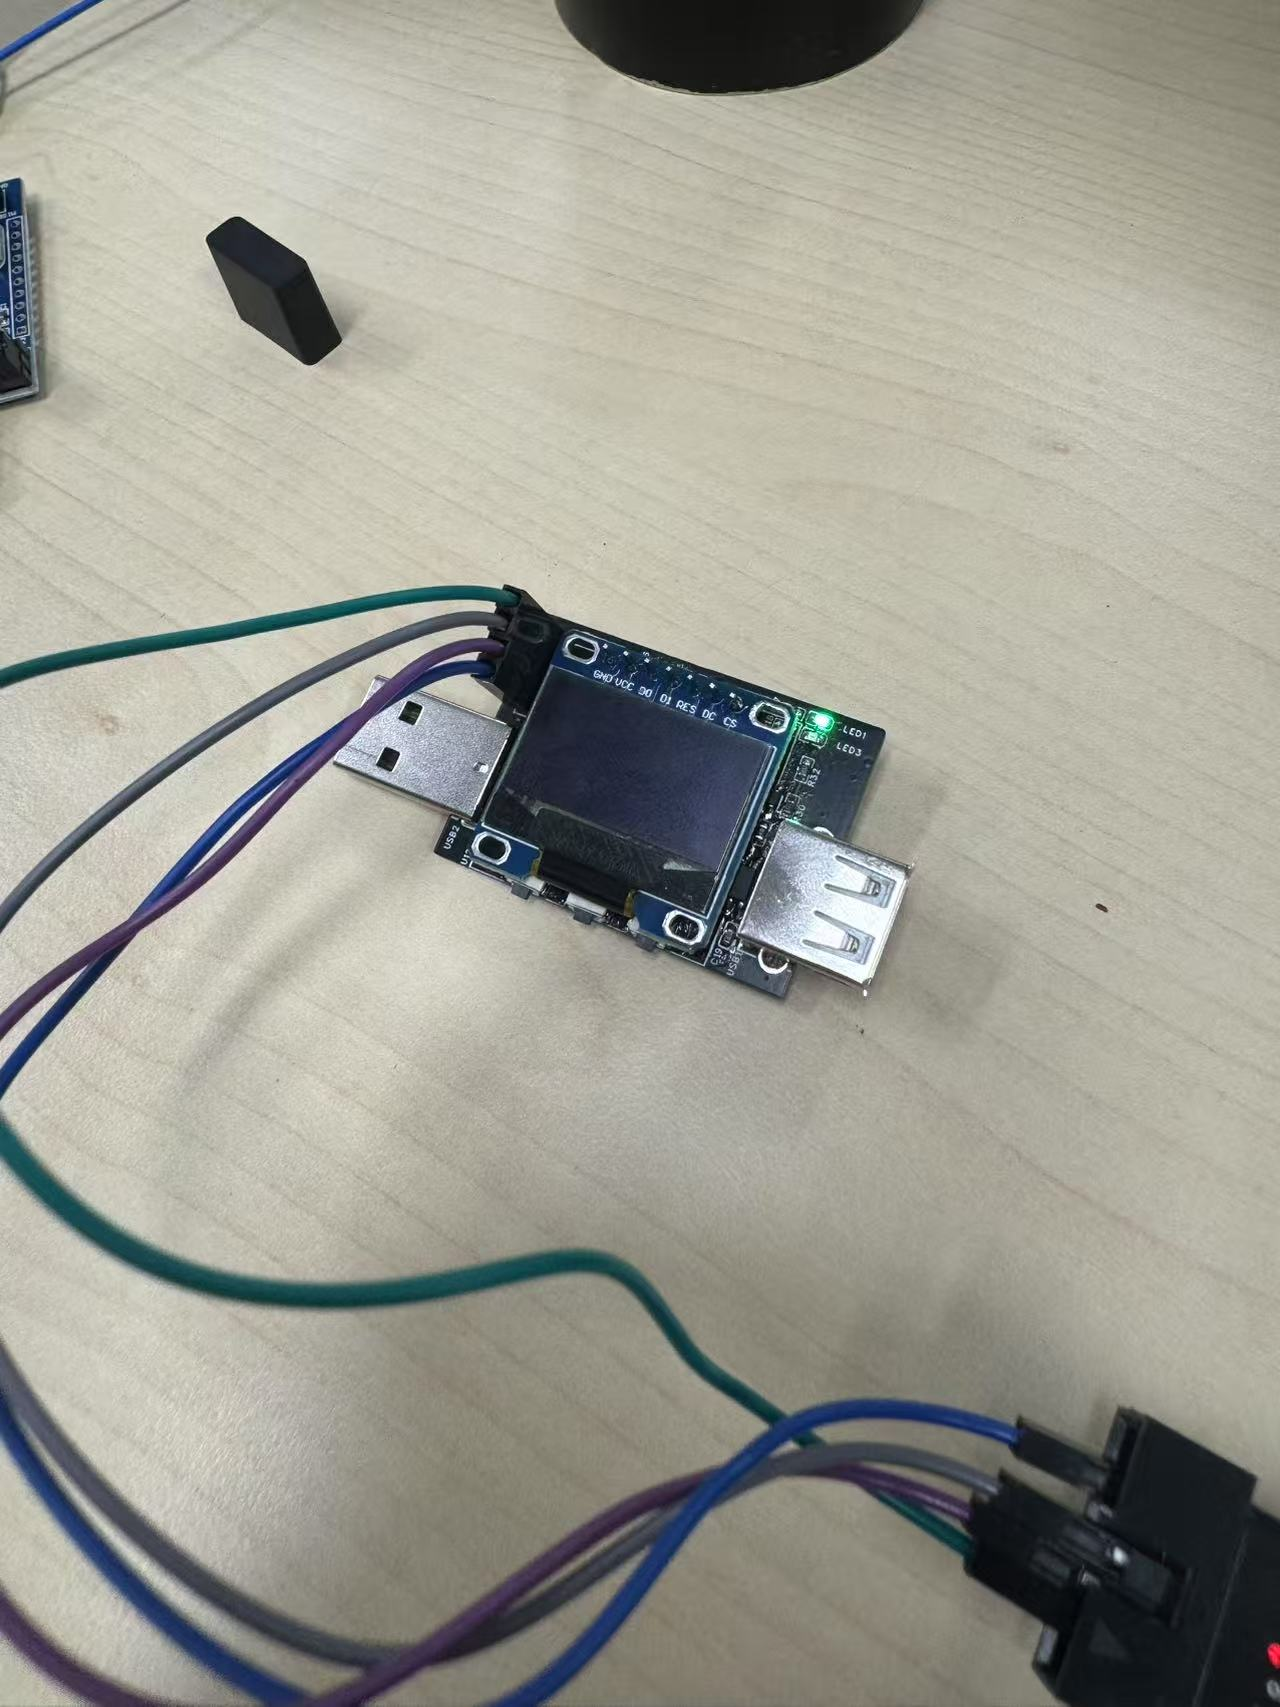
\includegraphics[width = .2\textwidth]{./figures/c73295887824945795a9509819d33a7.jpg}
\caption{焊接好的板子以及点亮的样子}
\end{figure}

后来我们放弃使用芯片专有的库来进行寄存器级别的开发,转而使用stm8s.h来进行开发,但是编译过程中一直无法找到库文件,后面查看了标程后把
标准库文件下载后放入项目文件夹,并添加了预编译路径,勉强可以使用stm8s.h进行开发。

在串口通信方面,我使用pip进行串口通信的读取,pyserial,但是python无法读到端口,到结题时也无法解决。
但我们把理论上能够实现的上位机python实现完成了。

但是我们成功实现了用按钮控制灯的亮灭
\begin{lstlisting}
/* Includes ------------------------------------------------------------------*/
#include "stm8s.h"

/* Private defines -----------------------------------------------------------*/
#define LED_G_GPIO_PORT      GPIOC
#define LED_G_GPIO_PIN       GPIO_PIN_6
#define BUTTON1_GPIO_PORT   GPIOC
#define BUTTON1_GPIO_PIN    GPIO_PIN_4
#define LED_R_GPIO_PORT      GPIOC
#define LED_R_GPIO_PIN       GPIO_PIN_7
#define BUTTON2_GPIO_PORT   GPIOC
#define BUTTON2_GPIO_PIN    GPIO_PIN_5

/* 按钮状态检测宏 */
#define BUTTON1_PRESSED()   (GPIO_ReadInputPin(BUTTON1_GPIO_PORT, BUTTON1_GPIO_PIN) == RESET)
#define BUTTON2_PRESSED()   (GPIO_ReadInputPin(BUTTON2_GPIO_PORT, BUTTON2_GPIO_PIN) == RESET)
#define DEBOUNCE_DELAY     1000  // 单位取决于Delay函数实现

void Delay(uint16_t nCount) {
  while(nCount--);
}

void main(void) {
  /* 初始化LED引脚:推挽输出 */
  GPIO_Init(LED_G_GPIO_PORT, LED_G_GPIO_PIN, GPIO_MODE_OUT_PP_LOW_FAST);

  GPIO_Init(LED_R_GPIO_PORT, LED_R_GPIO_PIN, GPIO_MODE_OUT_PP_LOW_FAST);
  /* 初始化按钮引脚:上拉输入(按钮按下接地) */
  GPIO_Init(BUTTON1_GPIO_PORT, BUTTON1_GPIO_PIN, GPIO_MODE_IN_PU_IT);
  GPIO_Init(BUTTON2_GPIO_PORT, BUTTON2_GPIO_PIN, GPIO_MODE_IN_PU_IT);
  while(1) {
    if(BUTTON1_PRESSED()) {          // 检测按钮按下
      Delay(DEBOUNCE_DELAY);        // 简单消抖
      if(BUTTON1_PRESSED()) {        // 确认有效按下
        GPIO_WriteReverse(LED_G_GPIO_PORT, LED_G_GPIO_PIN);  // 翻转LED状态
        while(BUTTON1_PRESSED());    // 等待按钮释放
      }
    }
    if(BUTTON2_PRESSED()) {          // 检测按钮按下
      Delay(DEBOUNCE_DELAY);        // 简单消抖
      if(BUTTON2_PRESSED()) {        // 确认有效按下
        GPIO_WriteReverse(LED_R_GPIO_PORT, LED_R_GPIO_PIN);  // 翻转LED状态
        while(BUTTON2_PRESSED());    // 等待按钮释放
      }
    }
  }
}

#ifdef USE_FULL_ASSERT

/**
  * @brief  Reports the name of the source file and the source line number
  *   where the assert_param error has occurred.
  * @param file: pointer to the source file name
  * @param line: assert_param error line source number
  * @retval : None
  */
void assert_failed(u8* file, u32 line)
{
  /* User can add his own implementation to report the file name and line number,
     ex: printf("Wrong parameters value: file %s on line %d\r\n", file, line) */

  /* Infinite loop */
  while (1)
  {
  }
}
#endif
\end{lstlisting}

其中推挽输出可能带动耗电量较大的原件,如继电器,发光二极管。

通过GPIO初始化管脚,其中管脚的地址都在PCB的原理图中可以找到。

需要设置按钮为上拉,此时按钮按下就会接地,这个信号可以被检测到用于控制灯。

然后通过在灯的脚上输出反转的电平,就可以实现灯的亮灭。

串口通信的思考理解:

芯片通过uart协议与上位机进行通信,stm8的tx管脚在PD5,rx在PD6。

\lstset{ %
backgroundcolor=\color{white},   % choose the background color
basicstyle=\footnotesize\ttfamily,        % size of fonts used for the code
columns=fullflexible,
breaklines=true,                 % automatic line breaking only at whitespace
captionpos=b,                    % sets the caption-position to bottom
tabsize=4,   % comment style
escapeinside={\%*}{*)},          % if you want to add LaTeX within your code
keywordstyle=\color{blue},       % keyword style
frame=single,
rulesepcolor=\color{red!20!green!20!blue!20},
% identifierstyle=\color{red},
language=python,
}
\begin{lstlisting}
    port_name = "COM3"
    ser = serial.Serial(
        port=port_name,
        baudrate=115200,
        bytesize=serial.EIGHTBITS,
        parity=serial.PARITY_NONE,
        stopbits=serial.STOPBITS_ONE,
        timeout=1
    )
\end{lstlisting}
通过这块可以打开COM3串口并且读取文件。

\subsection{串口实现}
上位机数据处理与可视化:
思路:
  \begin{enumerate}
    \item 初始化阶段

    加载配置文件,比如端口的参数、显示的样式等;初始化串口连接,将单片机与上位机进行串口的实现;

    \item 数据采集阶段

    STM8 实时采集USB的电压与电流数据;

    \item 数据处理阶段

    主要在Python中采用了serial和Matplotlib 实时绘制折线图。

    计算功率值:$P = V \times I$

    \item 界面展现阶段
    \begin{enumerate}
      \item 自动调整坐标轴范围保证数据可见,显示图形时横轴表示时间(最近 10 秒),纵轴显示三条曲线:电压、电流及功率,并定义了横轴和纵轴的名字
      \item 更新状态栏实时数值显示
    \end{enumerate}

  \end{enumerate}初始化阶段
问题:最终只能展现一条线,无法呈现三条线
\begin{figure}[H]
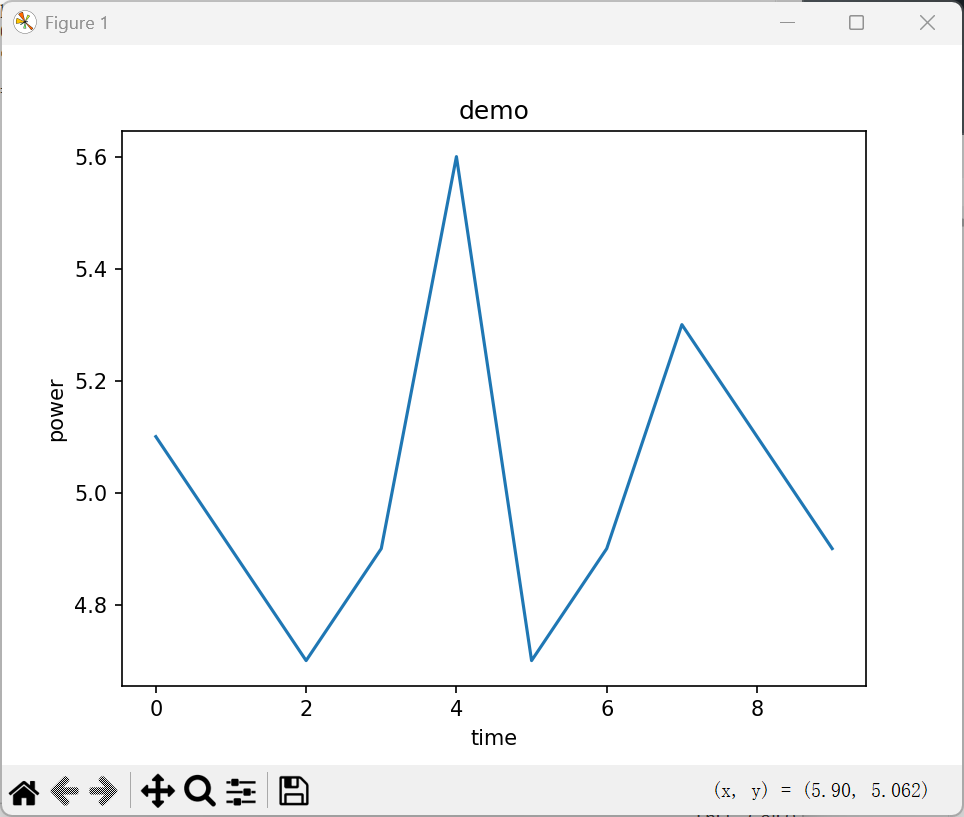
\includegraphics[width=.4\textwidth]{./figures/fig.png}
\end{figure}
\end{document}